\documentclass{report}
\usepackage{graphicx}
\usepackage{braket}
\usepackage[italian]{babel}
\usepackage{float}
\usepackage{wrapfig}
\usepackage{amsmath}
\usepackage{amssymb}
\usepackage{braket}
\usepackage{parskip}
\usepackage{cancel}
\usepackage{bbold}
\usepackage{upgreek}
\usepackage{hyperref}
\usepackage{caption}
\usepackage{tikz}
\usepackage{mathtools}
\DeclarePairedDelimiter{\ceil}{\lceil}{\rceil}

\usepackage{geometry}
\renewcommand{\figurename}{Figura}
\geometry{
	a4paper,
	total = {160mm,260mm},
	left = 21mm,
	top = 18mm,
}


\title{\textbf{\Huge Quantum Information}\\ {\Large \textbf{\textit{Appunti del corso}}}}
\author{\textit{Giuseppe Scordo,} \\ \textit{Stefano Mavilla,} \\ \textit{Damiano Trovato}}
\date{Anno Accademico 2025/26}

\begin{document}

\maketitle
\tableofcontents

\include{./chapters/introduzione}
\part{Teoria dell'Informazione Classica}
\include{./chapters/classica1}
\include{./chapters/classica2}
\include{./chapters/classica3}
\include{./chapters/classica4}
\include{./chapters/classica5}
\include{./chapters/classica6}
\include{./chapters/classica7}
\include{./chapters/classica8}

\part{Informazione Quantistica}
\chapter{Fondamenti di algebra lineare}
L'algebra lineare è il linguaggio fondamentale della meccanica quantistica, in cui gli stati fisici sono rappresentati come vettori in uno spazio di Hilbert complesso. Operatori hermitiani agiscono su questi vettori per rappresentare osservabili fisiche, mentre le probabilità di misura sono calcolate tramite prodotti scalari, rendendo la teoria quasi interamente formulabile in termini di algebra lineare. Introduciamo quindi i fondamenti di algebra linearre che saranno necessari per la comprensione del corso.



\section{Spazio di Hilbert e prodotto scalare}
Si dice \textbf{spazio di Hilbert} uno spazio vettoriale completo rispetto alla norma indotta dal prodotto scalare. Ci saranno utili nello studio dei sistemi quantistici, a causa dell'assioma 1 della meccanica quantistica.

\begin{center}
	\vspace{3pt}
	\textbf{\Large Assioma 1 della meccanica quantistica}\\
	\vspace{5pt}
	\it Ad ogni sistema fisico quantistico è associato uno spazio di Hilbert $\mathcal{H}$.\rm
\end{center}

Tutti gli spazi di Hilbert che andremo a trattare sono finiti, in quanto i sistemi su cui operiamo sono finiti.
Consideriamo lo \textbf{spazio di Hilbert} $\mathbb{C}^d$ dei vettori colonna sui numeri complessi. Un elemento di questo spazio di Hilbert, è del tipo

$$
\overline{v} =
\begin{pmatrix}
	v_1 \\
	v_2 \\
	\vdots \\
	v_d
\end{pmatrix},
\hspace{0.3cm} v_i \in \mathbb{C}
$$
È inoltre dotato del \textbf{prodotto scalare} $\braket{v|w} = \sum^{d-1}_{i=0}\bar{v_i}w_i$.
Nel contesto dei numeri complessi, $\overline v$ indica il coniugato complesso di $v$, ossia:
$$
v = a + ib, \qquad \overline v = a - ib
$$
%
Sia $\mathcal{H}$ è uno spazio di Hilbert arbitrario con $\dim(\mathcal{H} = d)$ finita, posso scegliere una \textbf{base ortonormale} $\left\{ \ket{e_i} \right\}^d_{i=1}$ di $\mathcal{H}$, ossia tale che:

$$
\braket{e_i|e_j}  = 
\begin{cases}
	1 & \text{se }i=j  \\
	0 & \text{se }i\neq j
\end{cases}
$$
%
Indichiamo i vettori di $\mathcal{H}$ con il simbolo $\ket{\psi}$ e $\bra{\psi}$ per il suo duale. $\ket{\psi}$ è un vettore colonna, mentre $\bra{\psi}$ è un vettore riga. 

\paragraph{Base ortonormale standard} Una base ortonormale particolare, è la \textbf{base ortonormale standard}.
La base ortonormale standard di un qualsiasi spazio di Hilbert $\mathcal{H}= \mathbb{C}^d$ è data dall'insieme di vettori
$$
\ket{0}=
\begin{pmatrix}
	1 \\
	0 \\
	\vdots \\
	0
\end{pmatrix}, \
\ket{1}=
\begin{pmatrix}
	0 \\
	1 \\
	\vdots \\
	0
\end{pmatrix}, \dots,\
\ket{d-1}=
\begin{pmatrix}
	0 \\
	0 \\
	\vdots \\
	1
\end{pmatrix}
$$

Se $\ket{\psi} = 
\begin{pmatrix}
	\psi_1 \\
	\psi_2 \\
	\vdots \\
	\psi_{d-1}
\end{pmatrix}
$, allora $\ket{\psi} = \sum^{d-1}_{i=0}\psi_i \ket{i}$, e il suo duale è:
$\bra{\psi} = \left(\overline{\psi}_0,\overline{\psi}_1,\dots,\overline{\psi}_{d-1} \right)$. 

\subsection{Disuguaglianza di Schwartz}
Il prodotto scalare soddisfa la seguente disuguaglianza, nota come disuguaglianza
$$\forall \ket{\Phi},\ket{\Psi} \in \mathcal{H} = \mathbb{C}^d, \hspace{0.2cm} \left|\braket{\Phi|\Psi} \right|^2 \le \braket{\Phi|\Phi} \cdot \braket{\Psi|\Psi}$$
E vale solo se: $$\ket{\Phi} = k\ket{\Psi}, \exists k \in\mathbb{C}$$

La norma indotta del prodotto scalare è $\left| \left| \Psi\right| \right| = \sqrt{\braket{\Psi|\Psi}}$, per cui possiamo riscrivere il lemma di Schwartz come:
$$\braket{\Phi|\Psi} = \left| \left|\Phi \right| \right| \cdot \left| \left|\Psi \right| \right|$$

\section{Mappe lineari e matrici}
Utilizziamo funzioni lineari $f$, con le seguenti proprietà:
\begin{enumerate}
	\item $f(\lambda x) = \lambda f(x)$,
	\item $f(x+y) = f(x) + f(y)$ 
\end{enumerate}

Dati $\mathcal{H}= \mathbb{C}^d, \mathcal{K} = \mathbb{C}^e$ spazi di Hilbert, $\textit{lin}(\mathcal{H},\mathcal{K})$ è l'insieme delle \textbf{mappe lineari} da $\mathcal{H}$ a $\mathcal{K}$.\\ Se fissiamo una base per $\mathcal{H}$ e una base per $\mathcal{K}$ allora ogni mappa di $\textit{lin}(\mathcal{H},\mathcal{K})$ può essere scritta come una matrice $d\times e$.

Quando la mappa lineare va dallo stesso spazio allo stesso spazio, si dice \textbf{endomorfismo}. Un esempio è $\textit{lin}(\mathcal{H},\mathcal{H}) $, che indicheremo più brevemente con $\textit{lin}(\mathcal{H})$. 


Una particolare mappa lineare $\mathcal{H} \to \mathcal{H}$ è l'identità $ \mathbb{1}$.

\subsection{Traccia}
La \textbf{Traccia} di $M \in \textit{lin}(\mathcal{H})$ si calcola scegliendo una base $\Sigma$ di $\mathcal{H}$ e sommando gli elementi della diagonale principale.
$$\text{tr}[M] = \sum_{i \in \Sigma} \braket{i|M|i}$$
La traccia  è un invariante  per cambiamenti di base e soddisfa 
$$\text{tr}[MN] = \text{tr}[NM],\hspace{0.4cm} \forall M\in \textit{lin}(\mathcal{H,K}),N\in \textit{lin}(\mathcal{K,H})$$

Se $M\in \textit{lin}(\mathcal{H})$ e $N = \ket{\Psi}\bra{\Psi}$ per $\ket{\Psi}\in \mathcal{H}$ allora 
$\text{tr}[MN]=\braket{\Psi|M|\Psi}$

\subsection{Autovettori e autovalori}
Se $M\in \textit{lin}(\mathcal{H})$ e $\exists\ket{\Psi}\in \mathcal{H}$ non nullo e $n \in \mathbb{C}$ t.c $M \ket{\Psi} = \lambda \ket{\Psi}$ allora $\ket{\Psi}$ è un \textbf{Autovettore} di $M$ con \textbf{Autovalore} $\lambda$.

Se $M\in \textit{lin}(\mathcal{H}_1,\mathcal{H}_2)$, dove $\mathcal{H}_1$ ha base $\Sigma_1$ e  $\mathcal{H}_2$ ha base $\Sigma_2$ allora 
$$M = \sum_{i \in \Sigma_1}\sum_{j \in \Sigma_2} M_{ij} \ket{i}\bra{j}\hspace{0.2cm} \text{e} \hspace{0.2cm} M_{ij} = \braket{i|M|j}$$

\subsection{Matrice trasposta coniugata (o aggiunta, o dagger)}
Sia  $M\in \textit{lin}(\mathcal{H}_1,\mathcal{H}_2)$, l'\textbf{operatore aggiunto} di $M$ è $M^\dagger$ (dagger), tale che $M^\dagger = \overline{M}^T$, e che

$$
\braket{\Psi|M|\Phi} = \overline{\braket{\Phi|M^\dagger|\Psi}}
$$

Ed inoltre
$$M^\dagger\in \textit{lin}(\mathcal{H}_2,\mathcal{H}_1) \qquad \text{e} \qquad M^\dagger = \sum_{i,j} \overline{M_{ij}} \cdot\ket{j}\bra{i}$$

Una proprietà interessante, è che, $\forall M \in \textit{lin}(\mathcal H_2, \mathcal H_3),\; N \in \textit{lin}(\mathcal H_1, \mathcal H_2)$, vale che $(MN)^\dagger = N^\dagger M^\dagger$.

\subsection{Operatori Hermitiani}
$M\in \textit{lin}(\mathcal{H})$ è \textbf{Hermitiano} (o autoaggiunto) se $M = M^\dagger$, cioè significa che $M$ ha elementi diagonali $M_{ii}$ reali e $M_{ij} = \overline{M_{ij}}$ per $i\neq j$.

$$\begin{pmatrix}
	1 & 1+i \\
	1-i & 0\\
\end{pmatrix}$$
Le matrici Hermitiane hanno autovalori reali e ammettono una base di autovettori.

\subsection{Teorema Spettrale}
Sia $M\in \textit{lin}(\mathcal{H})$ Hermitiana e $\dim (\mathcal{H} = d)$, allora 
$\exists \lambda_1\ge\lambda_2\ge\dots\ge \lambda_d \in \mathbb{R}$ e una base $\left\{\ket{\Psi}\right\} ^d_{i=1} $ t.c.
$$M = \sum^d_{i=1}\lambda_i \ket{\Psi_i}\bra{\Psi_i}\hspace{0.4cm} \text{e\hspace{0.4cm} $\left\{ \lambda\right\} ^d_{i=1} $ si chiama \textbf{Spettro di M}}$$

Questo teorema ci dice che una matrice hermitiana può essere diagonalizzata usando matrici unitarie e la matrice diagonale ha elementi reali.
\medskip
\\OSS: lo spettro è univocamente è univocamente determinato da $M$ ma gli autovalori potrebbero essere non unici se lo spettro è degenere.
\\esempio: $\mathbb{1} = \sum^d_{i=1}\ket{\Psi_i}\bra{\Psi_i}, \hspace{0.2cm} \forall \left\{ \ket{\Psi_i}\right\} ^d_{i=1}$ 

\medskip
Se $M$ è Hermitiano  (o unitario) e $f$ è una funzione a una variabile, allora
$$f(M) = \sum^d_{i=1} f(\lambda_i)\ket{\Psi_i} \bra{\Psi_i}$$
Ossia: bisogna che $f$ sia ben definita sullo spettro.

\subsection{Operatori Positivi}
$P \in \textit{lin}(\mathcal{H})$ è \textbf{Semidefinito positivo} (\textit{PSD}) oppure solo \textit{positivo} se
$$\forall \ket{\Psi} \in \mathcal{H}, \braket{\Psi|P|\Psi} \ge 0$$
\textbf{PSD($\mathcal{H})$} è l'insieme degli operatori $P\ge 0$ su $\mathcal{H}$
\medskip

$P \in \textit{lin}(\mathcal{H})$ è \textbf{Definitivo positivo} (\textit{PD}) $P > 0$ se $\forall \braket{\Psi|P| \Psi} > 0$

\medskip
\textit{PD($\mathcal{H}$)} è l'insieme degli operatori $P > 0$ su $\mathcal{H}$

\medskip 
\textbf{Lemma (caratterizzazione degli operatori PSD)}:

$P \in \textit{lin}(\mathcal{H})$ equivale a dire:
\begin{itemize}
	\item[\textbf{A.}] $P$ è \textit{PSD}, $\braket{\Psi|P|\Psi} \ge 0 \hspace{0.5cm} \forall\ket{\Psi}\in\mathcal{H}$ 
	\item[\textbf{B.}] $P$ è Hermitiano e i suoi autovalori sono \textbf{non negativi}
	\item[\textbf{C.}] $\exists M \in \textit{lin}(\mathcal{H,K}):P=M^\dagger M \hspace{0.3cm} \exists \mathcal{K}$ spazio di Hilbert
	\item[\textbf{D.}] $\forall Q \in PSD(\mathcal{H}),\  \text{tr}[PQ] \ge 0$
\end{itemize}

\subsubsection{Corollario}
Se $$P \in PSD(\mathcal{H}), M \in \textit{lin}(\mathcal{H,K})$$ allora $$MPM^\dagger \in PSD(\mathcal{K}) \qquad P\le Q \Leftrightarrow Q-P \ge 0$$
Questa nozione induce un ordinamento...

\subsubsection{Matrici Unitarie e Isometrie}
\begin{itemize}
	\item $V \in \textit{lin}(\mathcal{H,K})$ è \textbf{Isometria} se $V^\dagger V = \mathbb{1}$ (solo se $\dim(\mathcal{H}) \le\dim(\mathcal{K})$)
	
	\item $V\in \textit{lin}(\mathcal{H})$ è \textbf{Unitaria} se $U^\dagger U = UU^\dagger = \mathbb{1}$
	
\end{itemize}

Definiamo $U(\mathcal{H})$ l'\textbf{insieme delle matrici unitarie} su $\mathcal{H}$:
$$\textit{Isom}(\mathcal{H,K})$$ 
insieme delle matrici isometrie da $\mathcal{H}$ a $\mathcal{K}$

$P \in \textit{lin}(\mathcal{H})$ è una \textbf{Proiezione} se $P^2 = P$ e $P$ è Hermitiana.

Sia $$\left\{\ket{e_i} \right\}^d_{i=1}$$ base per l'immagine di una proiezione $P$, allora 
$$P = \sum^d_{i=1}\ket{e_i}\bra{e_i}$$

Supponiamo $M$ Hermitiana, allora $M = \sum^d_{i=1} \lambda_i \ket{\Psi_i}\bra{\Psi_i}$

\medskip
I proiettori sono $P_\lambda = \sum_{i=\lambda} \ket{\Psi_i}\bra{\Psi_i}$

\medskip
Se $\Lambda =$ insieme degli autovalori \underline{distinti}, allora $$M = \sum_{\lambda\in \Lambda} \lambda P_\lambda$$

In generale $$M\in\textit{lin}(\mathcal{H,K}) \quad \text{,} \quad M = \sum^r_{i=1} s_i\ket{e_i}\bra{f_i}$$
con $s_i\ge0$ autovalori, $r = \textit{rank}(M)$ ed $e_i,f_i$ basi di $\mathcal{H}$ e $\mathcal{K}$.

\newpage
\subsection{Prodotti tensoriali}
Def. $\mathcal{H,K}$ spazi di Hilbert, il loro \textbf{Prodotto tensoriale $\mathcal{H} \otimes \mathcal{K}$} è lo spazio di Hilbert che contiene tutte le combinazioni lineari di vettori della forma $v \otimes u, \hspace{0.2cm} v\in\mathcal{H}, w \in \mathcal{K}$
\begin{itemize}
	\item $(\alpha v) \otimes (\beta w) = \alpha\beta \cdot v\otimes w, \hspace{0.2cm} \forall\alpha,\beta \in \mathbb{C}$
	\item $(v_1 + v_2) \otimes w = v_1 \otimes w + v_2 \otimes w$
	\item $v + (w_1 \otimes w_2) = v \otimes w_1 + v \otimes w_2$
\end{itemize}
Il prodotto scalare è definito da
$$\braket{v_1 \otimes w_2 |v_2 \otimes w_2} = \braket{v_1|v_2} \otimes\braket{w_1|w_2}$$
Base di $\mathcal{H} \otimes \mathcal{K} \hspace{0.5cm} \left\{ \ket{i} \otimes\ket{j} \right\}, \ket{i}\in B_\mathcal{H}, \ket{j} \in B_\mathcal{K}$

\medskip
$\ket{\Phi}\ket{\Psi} = \ket{\Phi\Psi} = \ket{\Phi} \otimes \ket{\Psi}$

\medskip
$\ket{\Phi} ^{\otimes n} = \ket{\Phi} \otimes \dots \otimes \ket{\Phi} \hspace{0.5cm} \mathcal{H}^{\otimes n} = \mathcal{H} \otimes\dots\otimes\mathcal{H}$

\medskip
Se $M \in \textit{lin}(\mathcal{H}_1,\mathcal{H}_2)$ e $N \in \textit{lin}(\mathcal{K}_1,\mathcal{K}_2)$ allora
$$M\otimes N : \mathcal{H}_1 \otimes \mathcal{K}_1 \longrightarrow \mathcal{H}_2 \otimes \mathcal{K}_2 $$
$$(M \otimes N) (\ket{ \Phi} \otimes \ket{\Psi}) = M\ket{\Phi} \otimes N \ket{\Psi}$$
$$\textit{lin}(\mathcal{H}_1\otimes\mathcal{K}_1,\mathcal{H}_2\otimes\mathcal{K}_2) = \textit{lin}(\mathcal{H}_1,\mathcal{H}_2) \otimes \textit{lin}(\mathcal{K}_1,\mathcal{K}_2)$$
$$M = \sum_{i,j}M_{ij}\ket{i}\bra{j}, \quad N = \sum_{k,l} N_{kl} \ket{k}\bra{l}$$
$$M \otimes N = \sum_{i,j,k,l} M_{ij} N_{kl}\ket{i}\bra{j} \otimes \ket{k}\bra{l} = \sum_{i,j,k,l} M_{ij} N_{kl}\ket{ik}\bra{jl}$$

\textbf{Lemma 4.1}
\begin{description}
	\item[a.] $P \in \textit{PSD}(\mathcal{H}), Q \in \textit{PSD}(\mathcal{K}) \Rightarrow P \otimes Q \in \textit{PSD}(\mathcal{H}\otimes\mathcal{K})$
	\item[b.] $\forall M \in \textit{lin}(\mathcal{H}), N \in \textit{lin}(\mathcal{K}), \text{ tr}[M\otimes N] = \text{tr}[M]\text{tr}[N]$
	\item[c.] $\forall M \in \textit{lin}(\mathcal{H}), N \in \textit{lin}(\mathcal{K}), \text{ rank}(M\otimes N) = \text{rank}(M)\text{rank}(N)$
	\item[d.] $\ket{\Phi}\otimes z = z\ket{\Phi}, z \in \mathbb{C} \hspace{1cm}\mathcal{H} \otimes \mathbb{C}= \mathcal{H}$
	\item[e.] $M\otimes \ket{\Psi}: \mathcal{H} \longrightarrow \mathcal{H} \otimes \mathcal{K} \hspace{0.8cm} (M\otimes \ket{\Psi})\ket{\Phi} = M \ket{\Phi} \otimes \ket{\Psi}$
	
	\medskip
	$M\otimes \bra{\Psi}: \mathcal{H} \otimes \mathcal{K} \longrightarrow \mathcal{H} \hspace{0.8cm} (M\otimes \bra{\Psi}) (\ket{\Phi}\otimes\bra{\chi}) = \braket{\Psi|\chi} M \ket{\Phi} \otimes \in \mathcal{H}$
\end{description}



\section{Stati Quantistici}
$$\ket{0} = 
\begin{pmatrix}
    1 \\
    0 \\
\end{pmatrix}
\hspace{1cm}
\ket{1} = 
\begin{pmatrix}
    0 \\
    1 \\
\end{pmatrix}
$$
$$\ket{q} = \alpha\ket{0}+\beta\ket{1}=
\begin{pmatrix}
    \alpha \\
    \beta \\
\end{pmatrix}
\hspace{1cm} p(0)= \left|\alpha \right|^2, p(1)= \left|\beta \right|^2,\hspace{0.2cm} \left|\alpha \right|^2 +\left|\beta \right|^2 = 1
$$
\subsection{Spazi di Hilbert}
\textbf{Assioma 1:} Ogni sistema quantistico è associato ad uno spazio di Hilbert $\mathcal{H}$.

Se $\dim \mathcal{H} = d$ posso identificare $\mathcal{H}$ come $\mathbb{C}^d$ munito del prodotto scalare standard.
Un sistema quantistico associato a $\left(\mathbb{C}^d,<\cdot,\cdot> \right)= \mathcal{H}$ oìpuò essere pensato come avente $d$ possibili stati distinti.
\\Esempio: Lo spazio di Hilbert più banale è $\mathbb{C}^2$, associato ad un solo qubit , ed ha come base $\ket{0}$ e $\ket{1}$
\subsection{Stati Quantistici}
\textbf{Definizione Matrice Densità}: una \textbf{Matrice densità} è un operatore \textbf{semidefinito positivo}\\ $\rho \in \textit{PSD}(\mathcal{H})$ con traccia $\text{tr}[\rho]=1$.
Denotiamo l'insieme delle matrici densità su $\mathcal{H}$ con $$S(\mathcal{H})=\{\rho \in\textit{PSD}(\mathcal{H}:\text{tr}[\rho]=1\}$$

\textbf{Assioma 2}: Lo stato di un sistema quantistico con spazio di Hilbert $\mathcal{H}$ è descritto da una matrice densità.

\textbf{Stati classici}: Sia $\Omega$ un insieme di possibili risultati. Allora la collezione delle distribuzioni di probabilità su $\Omega$ è: $$P(\Omega)=\left\{p : \Omega\rightarrow\mathbb{R}_{\ge0}\quad|\quad\sum_{x \in \Omega}p(x)=1\right\}$$

Alcune volte $p_x:= p(x)$, inoltre $\left\{p_x \right\}_{x\in \Omega}$ è una distribuzione di probabilità.

Sia $\mathcal{H}$ spazio di Hilbert e supponiamo che $\left\{ \ket{x}:x \in \Omega \right\}$ sia una base di $\mathcal{H}$.
Allora possiamo associare ad ogni distrubuzione di probabilità $p \in P(\Omega)$ lo stato quantistico
$$\rho  = \sum_{x \in \Omega} p(x)\ket{x}\bra{x} \hspace{0.2cm} \in S(\mathcal{H})$$
Esempio: consideriamo la base standard dello spazio di Hilbert a un qubit, $\mathcal{H}= \mathbb{C}^2$ con base $\Omega = \{0,1\}$
$$\rho = p(0) \ket{0}\bra{0}+p(1) \ket{1}\bra{1}=
\begin{pmatrix}
    p(0) & 0\\
    0 & p(1) \\
\end{pmatrix}
$$
Analogamente, la base di $\mathcal{H} = \mathbb{C}^2$ è data da $\Omega = \{0,1,\dots,d-1\}$. (Nota: sost. i sigma con omega)

In generale se $\Omega$ è un insieme finito, scriviamo $\mathcal{H}= \mathbb{C}^d$ per denotare uno spazio di Hilbert ortonormale $\left\{ \ket{x}:x \in \Omega  \right\}$, i vettori di $\mathcal{H}$ sono combinazioni lineari \textit{"formali"} dei vettori della base
$$\mathcal{H} = \mathbb{C}^\Omega = \left\{ \ket{v} = \sum_{x\in \Omega} v_x \ket{x}:v_x \in \mathbb{C}\right\}$$
e il prodotto scalare è $\braket{v|w}=\sum_{x\in \Omega} \overline{v}_x w_x$

\medskip
\textbf{Definizione di Stato Classico}: Sia $\Omega$ un insieme finito. Uno stato quantistico $\rho \in S(\mathcal{H})$ su $\mathcal{H}= \mathbb{C}^\Omega$ è uno \textbf{Stato classico} se nella forma: $$\rho = \sum_{x\in \Omega}p(x)\ket{x}\bra{x}, \text{ con } p\in P(\Omega)$$
Esempio: Il lancio di una moneta: 
$$\rho = \frac{1}{2}\left( \ket{0} \bra{0}+ \ket{1}\bra{1}\right)= 
\frac{1}{2}
\begin{pmatrix}
    1 & 0\\
    0 & 1
\end{pmatrix}
$$
Gli stati classici sono matrici diagonali rispetto alla base computazionale.

\subsection{Stati Puri}
Dato $\ket{\Psi} \in \mathcal{H}$ con norma unitaria, ovviamente $||\ket{\Psi}|| = \braket{\Psi|\Psi}=1$ , non può essere associato alla matrice densità
$$\rho = \ket{\Psi} \bra{\Psi}$$

$\rho$ è una matrice densità, infatti $\rho \in$ PSD e tr$[\rho] = \text{tr}[\ket{\Psi}\bra{\Psi}]=\text{tr}[\braket{\Psi|\Psi}]=1$

%$\mathcal{H}$ (\textit{Lemma 0.2})

Definizione: uno \textbf{Stato puro} $\rho \in S(\mathcal{H})$ è tale se $\ket{\Psi} \in \mathcal{H}$ tale che $\rho = \ket{\Psi}\bra{\Psi}$. Uno stato non puro di dice \textbf{Stato Misto}.

C'è una ridondanza nella descrizione $\ket{\Psi}$ di uno stato (notazione di Dirac): moltiplicando per una fase globale la matrice densità \textbf{non cambia}. Sia $\ket{\Phi}= e^{i\theta}\ket{ \Phi}$ con $\Theta \in \mathbb{R}$, allora:
$$\ket{\Phi}\bra{\Phi} = (e^{i\theta}\ket{\Psi})(e^{i\theta}\bra{\Psi})^{\dagger} = 
e^{i\theta}\ket{ \Phi}e^{-i\theta}\bra{\Phi} = e^{i\theta-i\theta}\ket{ \Phi}\bra{\Phi}=
\ket{\Psi} \bra{\Psi}$$

\textbf{Lemma 1.3:} Sia $\rho\in S(\mathcal{H})$. Le seguenti condizioni sono equivalenti:
\begin{description}
    \item[a)] $\rho$ è uno stato puro
    \item[b)] $\rho$ ha rango 1
    \item[c)] $\rho$ è una proiezione
\end{description}

\textbf{Esempio}: In uno stato classico di dimensione 2 \textbf{non è puro}, la matrice densità sarà:
$$
\begin{pmatrix}
	\rho & 0\\
	0 & 1 - \rho
\end{pmatrix}
$$

Nel caso generale, sia $\ket{\psi}= \alpha\ket{0}+\beta\ket{1}$, con $\alpha, \beta \in \mathbb{C}$, $|\alpha|^2 + |\beta|^2=1$. Allora:
$$\rho= \ket{\psi}\bra{\psi}= 
\begin{pmatrix}
    \alpha \\
    \beta
\end{pmatrix}
\begin{pmatrix}
    \overline{\alpha} & \overline{\beta}
\end{pmatrix}
= \begin{pmatrix}
    \alpha^2 & \alpha\overline{\beta}\\
    \overline{\alpha}\beta & \beta^2
\end{pmatrix}
$$

\subsection{Stati quantistici generici}
Sia $\rho \in S(\mathcal{H}) \Rightarrow \rho \in \textit{PSD}(\mathcal{H}) \Rightarrow \rho$ è Hermitiana e i suoi autovalori sono non negativi, vale il \\\textbf{Teorema spettrale}:
$$\rho = \sum^d_{i=1}p_i \ket{\psi_i}\bra{\psi_i}$$
con $p_i\ge 0$ autovalori e $\left\{ \ket{\psi} \right\}^d_{i=1}$ base di autovettori.

Rispetto a questa base la matrice è diagonale e tr$[\rho] = \sum^d_{i=1} p_i = 1$
\\In altre parole gli autovalori $\left\{  p_i \right\}^d_{i=1}$ definiscono una distribuzione di probabilità: "abbiamo lo stato $\ket{ \Phi_i}$ con probabilità $\rho_i$".

%Interpretiamo lo stato $\rho$ come una situazione in cui abbiamo lo stato puro $\ket{\psi}$ con probabilità $p_i$.
\textbf{Osservazione}: Qualunque decomposizione $\rho = \sum^d_{i=1} p_i \ket{\psi_i}\bra{\psi_i}$ è simile alla nostra definizione di stato classico. La differenza cruciale è che per uno stato classico la matrice è diagonale rispetto alla base computazionale.
\medskip
\\Dato $\mathcal{H}$ di dimensione $d$ possiamo definire lo stato detto \textbf{Massimalmente Misto}: $$\tau_d=\frac{1}{d}\mathbb{1}$$
Questo stato può essere decomposto come:
$$\tau = \sum^d_{j=1} \frac{1}{d} \ket{e_j}\bra{e_j} \text{ di } \mathcal{H} \hspace{0.5cm} \left\{ \ket{e_j} \right\}^d_{j=1} \text{ base}$$
Ricordiamo che un insieme $X$ si dice \textbf{Convesso} se $\forall x_0,x_1 \in X$ e $\forall 0 \le t\le 1$, 
$$x_t = tx_1 + (1-t)x_0 \in X$$
Questo significa che tutti i punti del segmento tra $x_0$ e $x_1$ sono contenuti in $X$. Chiamiamo $x_t$ una \textbf{Combinazione Convessa} di $x_0$ e $x_1$. 

I \textbf{Punti estremi}, sono quelli che possono essere scritti solo come combinazioni banali ($t=0$ o $t=1$).

$P(\Sigma)$ è un insieme convesso che si chiama \textbf{Simplesso}. Dato un bit classico, $P(\{0,1\})$ è un segmento che congiunge $\begin{pmatrix}
    1 \\ 0
\end{pmatrix}
\text{ e }
\begin{pmatrix}
    0\\1
\end{pmatrix}
$, che sono due punti estremi.
\medskip
\\ \textbf{Lemma 1.6:} $S(\mathcal{H}) \subset \textit{lin}(\mathcal{H})$ è un insieme convesso e i suoi punti estremi coincidono con l'insieme dei suoi stati puri. 

\section{Qubit e Sfera di Bloch}
Le seguenti  matrici formano una base dello spazio vettoriale reale delle matrici hermitiane, sono dette \textbf{Matrici di Pauli}
$$
\mathbb{1}=
\begin{pmatrix}
    1 & 0\\
    0 & 1
\end{pmatrix}
, X =
\begin{pmatrix}
    0 & 1\\
    1 & 0
\end{pmatrix}
, Y=
\begin{pmatrix}
    0 & -i\\
    i & 0
\end{pmatrix}
, Z =
\begin{pmatrix}
    1 & 0 \\
    0 & -1
\end{pmatrix}
$$
\begin{itemize}
    \item $X,Y,Z$ hanno \textbf{Traccia 0} (\textit{traceless})
    \item Sono hermitiane e unitarie, pertanto $X^2=Y^2=Z^2=\mathbb{1}$
    \item $X,Y,Z$ hanno \textbf{Autovalori 1 e -1}
    \item $X,Y,Z$ si autocommutano e si semplificano ciclicamente
    $$XY = -YX, \hspace{0.2cm} YZ = -ZY,  \hspace{0.2cm} ZX = -XZ$$
    \item $X,Y,Z$ si moltiplicano ciclicamente:
    $$XY = iZ, \hspace{0.4cm} YZ = iX,  \hspace{0.4cm} ZX = iY$$ 
\end{itemize}
Anche la \textbf{traccia dei prodotti} ovviamente è uguale a 0.

Sia $\rho \in \textit{lin}(\mathbb{C^2})$ una matrice hermitiana arbitraria con tr$[\rho] = 1$
$$\rho = \frac{1}{2}\left( \mathbb{1} + xX + yY+zZ\right) = \frac{1}{2}
\begin{pmatrix}
    1+z & x-iy \\
    x+iy & 1-z
\end{pmatrix}, \quad \text{con}\  x,y,z\in \mathbb{R}$$
 
Siano $\lambda_1,\lambda_2 \in \mathbb{R}$ gli autovalori di $\rho$, allora $\lambda_1,\lambda_2 \ge 0$ e tr$[\rho]=1$
allora almeno uno tra $\lambda_1$ e $\lambda_2$ deve essere positivo. Quindi, $\rho \in \textit{PSD} \Leftrightarrow \lambda_1\lambda_2=\det(\rho)\ge0$
$$\det(\rho) = \frac{1}{4}\left( (1+z) (1-z) - (x-iy) (x+iy) \right) = \frac{1}{4}(1-x^2-y^2-z^2)$$
$$\rho \text{ è PSD } \Longleftrightarrow 1-x^2-y^2-z^2\ge 0 \Longleftrightarrow x^2+y^2+z^2 \le 1$$
$$ \Longleftrightarrow \vec{r}= (x,y,z) \text{ ha norma } ||\vec{r}|| \le1$$

Lo stato di un qubit è parametrizzato da una palla solida di raggio 1 ed è chiamata \textbf{Palla di Bloch} (\textit{Bloch Ball}), mentre il vettore $\vec{r}$ è chiamata \textbf{Vettore di Bloch}.

In che caso otteniamo uno stato puro? La risposta  viene data dal Lemma 1.2: se e solo se abbiamo un autovalore uguale a 1 e l'altro uguale a 0, così che $\det(\rho(\vec{r}))= 0$, il che è equivalente al fatto che $\vec{r}$ è unitario. Quindi gli stati puri di un qubit sono parametrizzati da una sfera unitaria su $\mathbb{R}^3$ chiamata \textbf{Sfera di Bloch}.

Lemma 2.1: Ogni $\rho \in S(\mathbb{C^2})$ di un qubit può essere scritto come
$$\rho = \frac{1}{2}\left( \mathbb{1} + xX + yY + zZ \right)$$
\begin{wrapfigure} {r}{0.35\textwidth}
    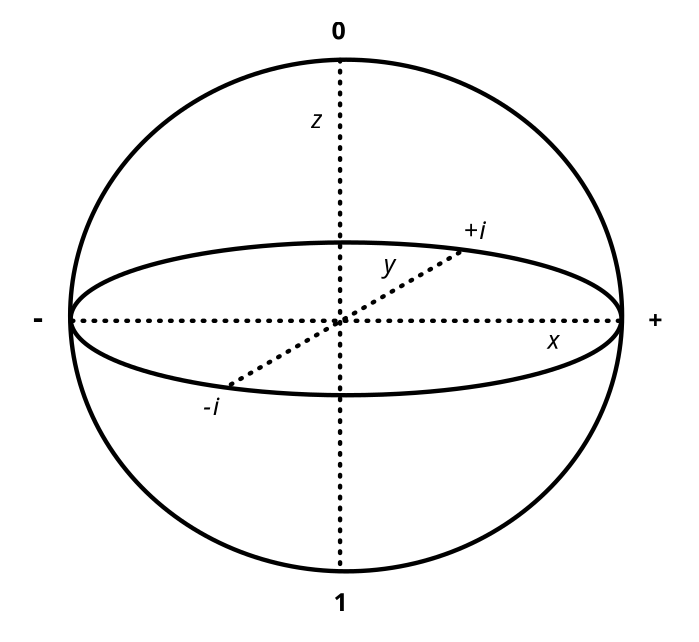
\includegraphics[width=1\linewidth]{images/Bloch.png}

\end{wrapfigure}
I punti interni rappresentano stati misti, in particolare il centro $\vec{r}=(0,0,0)$ corrisponde allo \textbf{Stato massimalmente misto} $$\rho(\vec{r})=\tau = \frac{\mathbb{1}}{2}$$
Un vettore $\vec{r}=(0,0,2p-1)$ sull'asse $\vec{z}$ con $p\in[0,1]$ corrisponde ad uno stato classico
$$\rho = \frac{1}{2}(\mathbb{1} + (zp-1)Z) = \frac{1}{2}
\begin{pmatrix}
    1+(2p-1) & 0\\
    0 & 1-(2p-1)
\end{pmatrix}
$$
$$
= \begin{pmatrix}
    p & 0\\
    0 & 1-p
\end{pmatrix}
$$
\newpage
Vediamo quali stati sono intersezione degli assi con la sfera:
\begin{itemize}
    \item Asse $\vec{z}$: \\$\vec{r}=(0,0,1)= \ket{0}$ , $\vec{r}=(0,0,-1)= \ket{1}$
    \item Asse $\vec{x}$: \\$\vec{r}=(1,0,0)= \ket{+}= \frac{1}{\sqrt{2}}(\ket{0} + \ket{1})$ , $\vec{r}=(-1,0,0)= \ket{- }= \frac{1}{\sqrt{2}}(\ket{0} - \ket{1})$
    \item Asse $\vec{y}$: \\$\vec{r}=(0,1,0)= \ket{+i}= \frac{1}{\sqrt{2}}(\ket{0} + i\ket{1})$ , $\vec{r}=(0,-1,0)= \ket{-i}= \frac{1}{\sqrt{2}}(\ket{0} - i\ket{1})$
\end{itemize}

Abbiamo ottenuto 3 diverse basi di $\mathbb{C^2}$, che chiamiamo basi $X,Y,Z$
\begin{itemize}
    \item I vettori della base $X$ sono gli autovettori $\ket{\pm}$ della matrice di Pauli $X$
    \item I vettori della base $Y$ sono gli autovettori $\ket{\pm i}$ della matrice di Pauli $Y$
    \item I vettori della base $Z$ sono gli autovettori $\ket{0},\ket{1}$ della matrice di Pauli $Z$
\end{itemize}

\section{Misurazioni}
Definizione: una \textbf{Misurazione} o \textbf{POVM} (\textit{Positive-Operator-Valued-Measure}) su uno spazio di Hilbert $\mathcal{H}$ con insieme dei risultati $\Omega$ è una collezione di operatori:
$$\mu=\left\{ \mu(x) \in \textit{PSD}(\mathcal{H}) \right\}_{x\in\Omega}\quad \text{tale che}\quad \sum_{x\in\Omega} \mu(x) = \mathbb{1}$$

Denotiamo con $\textit{Meas}(\mathcal{H},\Omega)$ l'insieme di tutte le misure su $\mathcal{H}$ con l'insieme dei risultati in $\Omega$, inoltre\\ $0\le\mu_x\le\mathbb{1}$ dove $\mu_x=\mu(x)$ 
(Notazione utilizzata) sono operatori che hanno autovalore $$\lambda:0\le\lambda\le1 \hspace{0.3cm} \forall x \in \Omega$$

\textbf{ASSIOMA 3 (Misurazioni)}

Quando eseguiamo una misurazione $\mu\in \textit{Meas}(\mathcal{H},\Omega)$ su uno stato quantistico $\rho\in S(\mathcal{H})$ osserviamo il risultato $x\in \Omega$ con probabilità $$p(x) = \text{tr}[\mu_x\rho]$$
Vediamo un esempio: con un singolo qubit consideriamo $\Omega= \{0,1\}$, e
$\mu=\{\mu_0,\mu_1\}:\mu_0=\ket{0}\bra{0},\mu_1=\ket{1}\bra{1}$, che definisce una misurazione. Misuriamo $\rho = \ket{\psi}\bra{\psi}$ per $\ket{\psi} = \ket{0}$

$$
    p(0)=\text{tr}[\mu_0\rho]=\text{tr}[\ket{0}\bra{0}\ket{0}\bra{0}] = 1
$$

$$
    p(1)=\text{tr}[\mu_1\rho]=\text{tr}[\ket{1}\bra{1}\ket{0}\bra{0}] = 0
$$

se invece $\ket{\psi} = \ket{+}$

$$
    p(0) = \text{tr}[\ket{0}\bra{0}\frac{1}{2}(\ket{0}+\ket{1})(\ket{0}+\ket{1})] = 
$$
$$
    = \frac{1}{2} \text{tr}\left[
    \begin{pmatrix}
        1 & 0\\
        0 & 0
    \end{pmatrix}
    \begin{pmatrix}
        1 & 1\\
        1 & 1
    \end{pmatrix}
    \right]
     = 
     \frac{1}{2} \text{tr}\left[
    \begin{pmatrix}
        1 & 0\\
        0 & 0
    \end{pmatrix}\right] = \frac{1}{2}
$$

analogamente $p(1) = \frac{1}{2}$.
\\Se consideriamo lo stato massimamente misto $\tau = \frac{1}{2}\mathbb{1}$
$$p(0)=\text{tr}[\ket{0}\bra{0}\frac{1}{2}\mathbb{1}] = \frac{1}{2}$$
e analogamente $p(1) = \frac{1}{2}$, cioè dalla misurazione non sappiamo distinguere $\ket{+}$ da $\tau$
\subsection{Misure rispetto a una base e misure proiettive}
Sia $\left\{\ket{e_x} \right\}_{x\in \Omega}$ una base arbitraria. Allora possiamo costruire una misurazione con l'insieme dei risultati $\Omega$, definendo
$$
    \mu_x = \ket{e_x}\bra{e_x} \hspace{0.3cm}\text{ per } x \in \Omega
$$
Quindi $\sum_{x\in\Omega}\mu_x = \sum_x \ket{e_x}\bra{e_x} = \mathbb{1}$ è una misura valida. Questo tipo di misura si chiama misura rispetto ad una base. In particolare, prendendo la base standard $\left\{ \ket{x} \right\}_{x\in\Sigma}$ otteniamo una misurazione rispetto alla base standard ($\Sigma$ insieme degli stati classici).
\medskip
\\ \textbf{Lemma 3.1} (\textit{Regola di Born}): Dato lo stato quantistico $\rho \in S(\mathcal{H})$, eseguendo una misura rispetto ad una base $\mu_x=\ket{e_x}\bra{e_x}$ osserviamo il risultato $x\in\Omega$ con probabilità $p(x)=\braket{e_x|\rho|e_x}$. Inoltre se $\rho = \ket{\psi}\bra{\psi}$ è uno stato puro $\ket{\psi}= \sum_{x\in\Omega}\Psi_x\ket{e_x}$ allora $p(x)=|\Psi_x|^2$
\medskip
\\ \textbf{Dimostrazione}: Poichè se $N = \ket{\psi}\bra{\psi}$ abbiamo che $$tr[MN]=\braket{\psi|M|\psi}$$ allora
$$p(x)= \text{tr}[\ket{e_x}\bra{e_x}\rho]=\braket{e_x|\rho|e_x}$$
Quando $$\rho = \ket{\psi}\bra{\psi}, \ket{\psi} = \sum_{x\in\Omega}\Psi_x\ket{\psi}$$ otteniamo $$p(x)=\braket{e_x|\psi} \braket{\psi|e_x}= |\braket{\psi|e_x}|^2=|\Psi|^2$$

Un caso più generale avviene quando gli operatori di misura $\mu_x$ sono tutte proiezioni, $\mu_x=P_x$. In tal caso abbiamo un operatore di misura proiettiva (\textit{PVM}). $\sum_{x\in\Omega}\mu_x = \mathbb{1}$, le immagini degli $\mu_x$ devono essere ortogonali e spannare tutto.
\subsection{Misurazione di qubit}
In generale scegliamo $\vec{r}=(x,y,z)$ con $||\vec{r}||=1$ e lo stato corrispettivo $-\vec{r}$. Allora 
$$\mu_{\vec{r},0}=p(\vec{r})=\frac{1}{2}
\begin{pmatrix}
    1+z & x-iy\\
    x+iy & 1-z
\end{pmatrix}\quad,\quad 
\mu_{-\vec{r},0}=p(-\vec{r})=\frac{1}{2}
\begin{pmatrix}
    1-z & -x+iy\\
    -x-iy & 1+z
\end{pmatrix}
$$
Se eseguiamo questa misura su uno stato quantistico con vettore di Bloch $\vec{s}=(x',y',z')$ allora la probabilità di ottenere $0$ è: $$p(0)= \frac{1}{2}+\frac{1}{2}\vec{r}\cdot\vec{s}=\frac{1}{2}+\frac{1}{2}(xx'+yy'+zz')$$ 

Geometricamente, $\vec{r}\cdot\vec{s}$ è la proiezione del vettore del Bloch...

Non esiste alcuno stato quantistico per cui entrambe le misure $X$ e $Z$ sono certe. Le misurazioni mappano uno stato quantistico in uno stato classico.

\textbf{Lemma 3.2}: Dato $\Omega$ insieme dei risultati classici, $\mathcal{H}$ spazio di Hilbert, supponiamo che per ogni $\rho\in S(\mathcal{H})$ esista una distribuzione di probabilità:
$$P_\rho\in P(\Omega): p\rho =p_1\rho_1+p_2\rho_2$$ per ogni stato misto
$\rho = p_1\rho_1+p_2\rho_2$. 

Allora, esiste un operatore di misura: $$\mu:\Omega\rightarrow\textit{PSD}(\mathcal{H}):\forall x\in\Omega, p\rho(x)=\textit{tr}[\mu(x)\rho]$$

\newpage
\section{Sistemi quantistici multipli}
Se $\mathcal{H}$ ha una base indicizzata $\ket{x_j}$ da $\ket{x_j}\in \Sigma_j$, allora il prodotto tensoriale $\mathcal{H}_1\otimes\mathcal{H}_2\otimes\dots\otimes\mathcal{H}_n$ ha la base prodotto $\ket{x_1,x_2,\dots,x_n}=\ket{x_1}\ket\otimes{x_2}\otimes\dots\otimes\ket{x_n}$
\medskip
\\ \textbf{ASSIOMA 4 (Sistemi multipli)}
\\Se abbiamo n sistemi quantistici con rispettivi spazi di hilbert $\mathcal{H}_1,\mathcal{H}_2,\dots,\mathcal{H}_n$, allora il sistema congiunto è associato allo spazio di Hilbert $\mathcal{H}_1\otimes\mathcal{H}_2\otimes\dots\otimes\mathcal{H}_n$
\medskip
\\ \textit{Notazione:} $A,B,C $ :Sistemi, $\hspace{0.5cm}\mathcal{H}_A,\mathcal{H}_B,\mathcal{H}_C$ : Spazi associati
\medskip
\\ $\rho_A,\rho_B,\rho_C,\rho_{AB},\rho_{BC},\rho_{AC},\rho_{ABC}$: Stati cogiuti
\medskip
\\$\Sigma_A,\Sigma_B,\Sigma_C$: Alfabeti di simboli
\medskip
\\ $\textit{lin}(A)= \textit{lin}(\mathcal{H}_A)$, $\hspace{0.3cm}S(A) = S(\mathcal{H}_A)$, $\hspace{0.3cm}\textit{PSD}(A)= \textit{PSD}(\mathcal{H}_A)$
\medskip
\\ $\mu_A\in\textit{Meas}(\mathcal{H}_A,\Omega)$, $\hspace{0.5cm}\Sigma_{AB}= \Sigma_A\times\Sigma_B$
\medskip
\\ \textit{Defizione}: $A,B$ stati quabtistici. Gli stati  nella forma $\rho=\rho_A\otimes\rho_B,\rho_A\in S(A),\rho_B\in S(B)$ si chiama \textbf{Stato prodotto}. Uno stato che non è prodotto si dice \textbf{Stato correlato}.
\\Se abbiamo $N$ sistemi, $\rho_{A_1,\dots,A_n}\in S(A_1,\dots,A_n)$ è uno stato prodotto se $\rho_{A_1,\dots,A_n}=\rho_{A_1}\otimes\dots\otimes\rho_{A_n},\hspace{0.3cm}\rho_{A_i}\in S(A_i)$

\textbf{Esempio}: Alice e Bob hanno un qubit ciascuno,   $\mathcal{H}_A = \mathcal{H}_b = \mathbb{C}^2 \ \Rightarrow\  \mathcal{H}_A\otimes\mathcal{H}_B \cong
\mathbb{C}^4$
\begin{enumerate}
    \item Essi potrebbero condividere uno degli stati base: $\ket{00},\ket{01},\ket{10},\ket{11}$, che corrispondono a stati puri e classici;
    \item Potrebbero avere $\ket{+}_A\ket{+}_B= \frac{1}{2}\left( \ket{00}+\ket{01}+\ket{10}+\ket{11} \right)$, che corrisponde ad uno stato \textbf{puro} ma non classico;
    \item Uno stato classico \textbf{non prodotto} si dice \textbf{Massimamente correlato} e corrisponde a 2 bit che si trovano nello stato $\ket{00}$ o $\ket{11}$ con probabilità uniforme:
    
    $$
    	\sigma_{AB} = \frac{1}{2}(\ket{00}\bra{00} + \ket{11}\bra{11})
    $$
    
    Esprimendolo nella base ${\ket{00},\ket{01},\ket{10},\ket{11}}$ otteniamo:
    $$
        \begin{pmatrix}
            1 &0 &0 &0\\
            0 &0 &0 &0\\
            0 &0 &0 &0\\
            0 &0 &0 &1
        \end{pmatrix}
    $$
    \item  Uno stato non classico e non prodotto si dice \textbf{Massimamente entangled} 
    $$\ket{\Phi^+}_{AB}=\frac{1}{\sqrt{2}}(\ket{00}+\ket{11})$$
    $$\rho_{AB}=\ket{\Phi^+}_{AB}\bra{\Phi^+}_{AB}
    =\frac{1}{2}(\ket{00}\bra{00}+\ket{00}\bra{11}+\ket{11}\bra{00}+\ket{11}\bra{11})= \frac{1}{2}
        \begin{pmatrix}
            1 & 0 & 0 & 1 \\
            0 & 0 & 0 & 0 \\
            0 & 0 & 0 & 0 \\
            1 & 0 & 0 & 1
        \end{pmatrix}
        =
    $$
    $$=\frac{1}{2}(\ket{0}\bra{0}\otimes\ket{0}\bra{0}+\ket{0}\bra{1}\otimes\ket{0}\bra{1}+\ket{1}\bra{0}\otimes\ket{1}\bra{0}+\ket{1}\bra{1}\otimes\ket{1}\bra{1})$$
\end{enumerate}

\textbf{Proprietà}:
$$
\ket{ab}\bra{cd} = (\ket{a}\otimes\ket{b})(\bra{c}\otimes\bra{d}) = \ket{a}\bra{c}\otimes\ket{b}\bra{d}
$$




\newpage
\section{Traccia Parziale}
Sia $\mu_A=\{\mu_A(x)\}_{x\in\Omega} \in \textit{Meas}\{A,\Omega\}$ una misurazione che Alice vuole effettuare sul suo sistema.\\
Supponiamo che Alice e Bob condividano uno stato quantistico ma non possano comunicare. Esiste un modo per avere solo lo stato $\rho_A$?
\medskip\\
La maniera più naturale di estendere questa misurazione al sistema $AB$ è considerare la misurazione Globale che esegue 
$\mu_A$ su $A$ e non fa nulla su $B$:

$$
    \mu_A\otimes\mathbb{1}_B=\{\mu_A(x)\otimes\mathbb{1}_B:x\in\Omega\}
$$

È una misurazione valida?
\begin{description}
    \item[i]    $\sum_{x\in\Omega}(\mu_A(x)\otimes\mathbb{1_B})=\left(\sum_{x\in A}\right)\otimes\mathbb{1}_B =\mathbb{1}_A\otimes\mathbb{1}_B=\mathbb{1}_{AB}$
    \item[ii]   $\mu_A(x)\otimes\mathbb{1}_B$ è PSD $\forall x \in \Omega$, il loro prodotto è PSD
\end{description}

In generale se Alice e Bob eseguono $\mu_A$ e $\mu_B$, rispettivamente con insieme dei risultati $\Omega_1$ e $\Omega_2$, corrispondono ad una misurazione sul sistema globale

$$
    \mu_A\otimes\mu_B:=\left\{ \mu_A(x)\otimes\mu_B(y) :(x,y)\in \Omega_1 \times\Omega_2 \right\}
$$

Si osservi che in tal caso, le sole probabilità dei risultati di Alice non dipendono da quelle dei risultati di bob
\medskip\\
Adesso vogliamo ricostruire una descrizione appropriata dello stato di ALice quando il sistema globale si trova nello stato $\rho_{AB}$. Vorremmo che:




\chapter{Quantum information processing}

\section{Quantum information processing}
Che operazioni possono essere fati su stati quantistici? Quando si applica un operatore su uno stato quantistisco, si effettua una operazione del tipo
\begin{equation}
\ket\psi \to U\ket\psi,
\end{equation}
%
o nel caso delle matrici di densità:
\begin{equation}
	\ket\psi\bra\psi \to U\ket\psi\bra\psi U^\dagger.
\end{equation}

\subsection{Evoluzione temporale}
Lo stato di un sistema quantistico $\ket{\psi_t}$ al tempo $t$, evolve secondo un Hamiltoniana $H(t)$.
\begin{equation}
\frac{d\ket{\psi_t}}{dt} = -i H(t)\ket{\psi_t}
\end{equation}

Noto lo stato di partenza $\ket{\psi_0}$ , otteniamo un equazione differenziale la cui soluzione determina lo stato $\ket{\psi_0}$ a tutti gli istanti $t$. La soluzione è tale che $\ket{\psi_t} = U_t\ket{\psi_0}$. Viceversa, data una mappa unitaria $U \in \textit{lin}(\mathcal H)$ esiste una Hamiltoniana $H(t)$ per $H(1) = U$.

Tutte le trasformazioni, in meccanica quantistica, coincidono con operazioni unitarie. In computazione quantistica, questo si traduce in gate ($X$, $Z$, $CNOT$).

\section{Operazioni sugli stati}
Queste operazioni sugli stati sono modellate tramite mappe lineari.
Vale quindi che
\begin{equation}
\phi_{A\to B}(\sum_i p_i\rho_i) = \sum_i p_i \phi_{A\to B}(\rho_i)
\end{equation}

\subsection{Superoperatori e proprietà}
Un superoperatore è un operatore lineare che agisce su altri operatori, mappando operatori lineari ad altri operatori.

Dati i sistemi quantistici $A, \ B$, un superoperatore da $A$ a $B$ è una mappa lineare da $\phi _{A \to B} : \textit{Lin}(A) \to \textit{Lin}(B)$. Se $A = B$, usiamo la notazione $\phi_A = \phi_{A\to A}$.

Alcuni superoperatori, sono:
\begin{itemize}
	\item \textbf{Superoperatore identità}
	\item \textbf{Traccia parziale}
	\item \textbf{Le isometrie}
\end{itemize}


Inoltre, è possibile comporre superoperatori $A \to B, B \to C$ per ottenere un superoperatore $A \to C$. 
Inoltre, il prodotto tensoriale $\phi_{A\to B} \otimes \psi_{C\to D} = AC \to BD$. 

\subsection{Mappe positive}
Un superoperatore $\phi_{A \to B}$ è una \textbf{mappa positiva} se $\forall P_A \in PSD(A)$ si ha $\phi_{A \to B} \in PSD(B)$.

\paragraph{Lemma sulla composizione di mappe positive} La composizione di mappe positive è una mappa positiva. Questa è la circostanza in cui più gate vengono posti uno dopo l'altro su una linea quantistica.

\paragraph{E sul prodotto tensoriale di mappe positive?}
Il prodotto tensoriale di mappe positive non è una mappa positiva!
Ad esempio, \bf INSERIRE ESEMPIO DELLA LEZIONE\rm


Abbiamo quindi bisogno di una condizione più forte, per mantenere la positività, nota come completa positività. 

Un superoperatore ... è una mappa completamente positiva (CP) se $\forall$ sistema di riferimento $R$, il superoperatore $\phi_{A \to B} \otimes I_R$ è positivo.
\begin{equation}
CP(A,B) = \{\text{superoperatori $CP$ da $A$ a $B$}\}, \quad CP(A,A) =
\end{equation}


\section{Canali quantistici}
...


\begin{center}
	\vspace{3pt}
	\textbf{\Large Assioma 5 dell'informazione quantistica}\\
	\vspace{5pt}
	\it L'insieme delle possibili operazioni da un sistema quantistico $A$ in un altro $B$ è l'insieme dei canali quantistici $C(A,B)$.\rm
\end{center}


\chapter{Misurare distanze ed errori}

Dati due stati quantistici $\rho$ e $\sigma$, quanto facilmente possiamo distinguerli con una misura?

\section{Metrica}
È necessario introdurre una metrica per valutare la distanza tra due stati.
Una \textbf{metrica} da un insieme (di stati quantistici) $S(\mathcal H)$ è una funzione 
\begin{equation}
d: S(\mathcal H) \times S(\mathcal H) \to \mathbb{R}_{\geq 0}, \text{ tale che}
\end{equation}
%
valgono le seguenti proprietà:
\begin{enumerate}
	\item $d(\rho, \sigma)$ ...
	\item ...
	\item ...
\end{enumerate}

\section{Norma 1 (o \textit{Trace norm})}
Una prima metrica può essere la \bf norma 1\rm. Sia $M \in Lin(\mathcal{H}, \mathcal K)$, la trace norm (o norma 1) di $M$ è la somma dei valori singolari di $M$.

\paragraph{Proprietà della trace norm}
Sia $M \in Lin(\mathcal H, \mathcal K)$, allora:
\begin{enumerate}
	\item $\|M\|_1 = tr[\sqrt{M^\top M}]$
	\item $\|M\|_1 = \|M^\dagger\|_1 = \|M^\top|_1 =\|\overline M\|_1$
	\item Se $V, \,W$ sono isometrie, $\|VMW\|_1 = \|M\|_1$
	\item Se $\mathcal H = \mathcal K$ e $M = M^\dagger$ ha spettro $\lambda_1, \dots, \lambda_m$, allora $\|M\|_1 =\displaystyle\sum_{i=1}^m |\lambda_i|$.
\end{enumerate}
%
Osserviamo che, se $\rho \in S(\mathcal H)$, allora $\|\rho\|_1 = 1$.

\subsection{Trace distance - metrica}
Date $\rho, \,\sigma \in S(\mathcal H)$, la \textbf{trace distance} tra $\rho, \, \sigma$ è

\begin{equation}
T(\rho, \sigma) \coloneqq \frac{1}{2}\|\rho - \sigma \|_1
\end{equation}

La trace distance gode di alcune proprietà. Siano $\rho, \, \sigma \in S(\mathcal H)$, allora:
\begin{enumerate}
	\item Se $\rho - \sigma$ ha autovalori $\lambda_1, \dots, \lambda_m$, possiamo calcolare la trace distance come
	\begin{equation}
		T(\rho, \sigma) = \sum _{i = 1, \lambda_i > 0}^n \lambda_i
	\end{equation}
	\item $T(\rho, \sigma) = \max_{0 \leq Q \leq 1} \mathrm{tr}[Q(\rho - \sigma)]$, e il massimo si ottiene quando $Q$ è una proiezione.
	
\paragraph{Dimostrazione proprietà 1}
\paragraph{Dimostrazione proprietà 2}

\subsection{Esempi di calcolo della trace distance}
$\rho_{AB} = \ket{\phi_{AB}^+} \bra{\phi_{AB}^+}$, $\sigma_{AB} = \frac{1}{2}\left( \ket{00}\bra{00} + \ket{11}\bra{11} \right)$

inserire calcolo...
\end{enumerate}

\subsubsection{Altre proprietà sulla trace distance}
\begin{enumerate}
	\item $0 \leq T(\rho, \sigma) \leq 1$, ed è uguale a zero se $\rho = \sigma$;
	\item Invariante per isometrie;
	\item Se $\rho_{AB} \in S(AB)$, allora $T(\rho_A, \sigma_A) \leq T(\rho_{AB}, \sigma_{AB})$, ossia è monotona sulla traccia parziale;
	\item Se $\phi_{A\to B} \in C(A,B)$ e $\rho_a, \sigma_a \in S(A)$. Allora 
\end{enumerate}
Le isometrie non fanno variare la trace distance. Osserviamo invece che la traccia parziale può causare una perdita di distinguibilità tra i due stati. 

\subsection{Teorema di Helstrom}

Dati $\rho,\, \sigma \in S(\mathcal H)$ matrici densità. Supponiamo di aver ricevuto $\rho, \, \sigma$ con una probabilità uniforme $\dfrac{1}{2}$. Allora la probabilità massima di identificare lo stato corretto eseguendo una misurazione con due risultati è \begin{equation}
p_{\max} = \frac{1}{2} + \frac{1}{2}T(\rho, \sigma)
\end{equation}.

\subsection{Cosa succede su stati classici?}
Se $p_x, \, q_x$ sono distribuzioni di probabilità su un sistema classico $X$ con matrici densità $\rho(x) = \sum_x p_x(x) \ket x \bra x$, $\sigma(x) = \sum_x q_x(x) \ket x \bra x$, allora la trace distance coincide con 

\begin{equation}
T(p_x, q_x) = \frac{1}{2} \sum_x |p_x(x - q_x(x))|,
\end{equation}
%
ossia con la distanza statistica su distribuzioni di probabilità.

\subsection{E su stati puri?}
Se $\ket\phi, \, \ket\psi \in \mathcal H$ e $\rho = \ket\phi \bra\phi$, allora

\begin{equation}
T(\rho, \sigma) = \sqrt{1 - |\braket{\phi\lvert\psi}|^2} 
\end{equation}
%
dove $\braket{\phi \lvert \psi} = \cos\theta$, con $\theta$ angolo tra $\phi, \, \psi$.

Inoltre, vale anche che 
\begin{equation}
|\braket{\phi \lvert \psi} | = \sqrt{\braket{\phi \lvert \psi}\braket{\psi \lvert \phi}} = \sqrt{\mathrm{tr}[\rho\sigma]}
\end{equation}

\subsection{Fidelity}
La fidelity tra $\rho, \, \sigma$ è definita come

\begin{equation}
F(\rho, \sigma) := \|\sqrt\rho\sqrt\sigma \|_1
\end{equation}

\paragraph{Osservazioni}

\end{document}